\documentclass[journal]{IEEEtran}
\usepackage{amsmath,amssymb,amsfonts}
\usepackage{graphicx,textcomp,xcolor,booktabs,multirow,url,hyperref,balance}

\begin{document}
\title{From SOC Alerts to News Articles: How Well Do Fine-Tuned LLMs Transfer Across Domains?}
\author{
\IEEEauthorblockN{Nutthakorn Chalaemwongwan}
\IEEEauthorblockA{Department of Computer Engineering, KOSEN-KMITL\\
King Mongkut's Institute of Technology Ladkrabang\\
Bangkok, Thailand\\
nutthakorn.ch@kmitl.ac.th}
}
\maketitle

\begin{abstract}
Fine-tuned LLMs achieve impressive in-domain performance, but practical deployment requires understanding cross-domain generalization. We train Qwen2.5-0.5B and Qwen2.5-7B on AG News (4-class news classification) and evaluate both in-domain and cross-domain transfer to GoEmotions (28-class emotion detection). In-domain, both models achieve strong performance: 0.5B reaches 88.72\% F1 and 7B reaches 91.06\% F1 on AG News. Cross-domain, transfer is \textbf{absolute zero}: the AG News-trained 0.5B model produces 0.0\% F1 on GoEmotions, generating news category labels (``Sports'': 39.8\%, ``Sci/Tech'': 5.0\%) for emotion-laden text. More intriguingly, the model also generates \emph{emotion-like labels not in its training data} (``Disgusted'': 9.4\%, ``Anger'': 5.6\%, ``Sad'': 5.2\%), revealing partial pre-training vocabulary leakage during cross-domain inference---a phenomenon absent during in-domain evaluation. We formalize this as \emph{domain-locked classification}: fine-tuning creates models that can only meaningfully classify inputs matching the training distribution. Task entropy $H(Y)$ predicts in-domain ML performance: DT drops from 87.4\% ($H=1.24$) to 17.3\% ($H=3.75$) across 4 domains, validating the entropy-based decision framework from P8. Our results establish that fine-tuned LLMs require separate models per domain.
\end{abstract}
\begin{IEEEkeywords}
cross-domain transfer, domain lock-in, multi-domain evaluation, task entropy, LLM generalization
\end{IEEEkeywords}

\section{Introduction}
Most LLM fine-tuning studies evaluate within a single domain. This creates a blind spot: does a model trained on news classification work for emotion detection? Can a cybersecurity model triage legal documents?

We address this with two complementary experiments:
\begin{enumerate}
\item \textbf{In-domain}: Train and test on AG News at two model scales (0. We use AG News (4-class news, $H = 2.0$ bits) as a controlled proxy to isolate the target phenomenon from domain-specific confounds. Its balanced distribution and established benchmark status enable clean ablation.5B, 7B).
\item \textbf{Cross-domain}: Train on AG News, test on GoEmotions (fundamentally different task).
\end{enumerate}

The cross-domain experiment reveals \textbf{absolute zero transfer}: the model produces 0.0\% F1, generating news labels for emotional text. But the predicted vocabulary reveals a surprising phenomenon: partial pre-training knowledge leaks through, producing emotion labels (``Disgusted,'' ``Anger'') that were never in the fine-tuning data and never appear during in-domain inference.

Combined with traditional ML baselines across 4 domains, we validate the entropy-based decision framework from P8~\cite{p8}: task entropy $H(Y)$ predicts when LLMs are necessary and when simpler methods suffice.

Our contributions:
\begin{enumerate}
\item Demonstration that cross-domain transfer is \textbf{zero} for fine-tuned 0.5B models---complete domain lock-in.
\item Discovery of \textbf{cross-domain vocabulary leakage}: pre-training knowledge surfaces during out-of-distribution inference but not during in-domain use.
\item \textbf{Model scale comparison}: 7B achieves +2.3 F1 points over 0.5B in-domain (91.1\% vs.\ 88.7\%).
\item \textbf{Multi-domain entropy validation}: ML performance degrades from 87.4\% to 17.3\% as $H$ increases from 1.24 to 3.75 bits.
\end{enumerate}

\section{Related Work}

\subsection{Transfer Learning in NLP}
BERT~\cite{devlin2019} demonstrated pre-training + fine-tuning transfers knowledge across tasks. T5~\cite{raffel2020} unified NLP as text-to-text, achieving cross-task transfer. Gururangan et~al.~\cite{gururangan2020} showed domain-specific pre-training improves downstream performance but did not evaluate cross-domain transfer \emph{after} fine-tuning. LoRA~\cite{hu2022} and QLoRA~\cite{dettmers2023} enable efficient adaptation, but cross-domain properties remain unstudied.

\subsection{Catastrophic Forgetting}
McCloskey and Cohen~\cite{mccloskey1989} first documented catastrophic interference. Kirkpatrick et~al.~\cite{kirkpatrick2017} proposed EWC. Luo et~al.~\cite{luo2023} showed fine-tuning erases general LLM capabilities. Our work quantifies: fine-tuning on 5K news samples completely eliminates emotion classification ability in 0.5B models.

\subsection{Multi-Domain NLP}
Sun et~al.~\cite{sun2023} compared GPT-4 vs.\ fine-tuned models but not cross-domain. HELM~\cite{liang2022} evaluates diverse tasks with base models. Ferrag et~al.~\cite{ferrag2024} surveyed cybersecurity LLMs. Aghajanyan et~al.~\cite{aghajanyan2021} showed fine-tuning operates in low-dimensional subspaces, explaining why cross-domain transfer fails. Muennighoff et~al.~\cite{muennighoff2023} and Sanh et~al.~\cite{sanh2022} showed multitask training enables zero-shot generalization---but only for base models, not fine-tuned ones. Our companion studies~\cite{p3,p21} document label hallucination and model size effects. We provide the first systematic \emph{fine-tuned} cross-domain evaluation on UNSW-NB15~\cite{moustafa2016} and general NLP datasets.

\textbf{Novelty gap.} No prior work has (1)~quantified cross-domain transfer loss for fine-tuned LLMs on classification, (2)~discovered vocabulary leakage during out-of-distribution inference, (3)~compared model scale effects on domain lock-in, or (4)~validated entropy-based decision frameworks across 4 domains.

\section{Experimental Setup}

\subsection{Domains and Datasets}

\begin{table}[h]
\centering
\caption{Cross-domain evaluation suite: AG News and GoEmotions with their class counts, entropy, and domain characteristics}
\label{tab:domains}
\begin{tabular}{llrccc}
\toprule
\textbf{Domain} & \textbf{Dataset} & \textbf{K} & $\mathbf{H(Y)}$ & \textbf{DT} & \textbf{SVM} \\
\midrule
Cybersecurity & SALAD & 8 & 1.24 & .874 & .909 \\
News & AG News & 4 & 2.00 & .556 & .882 \\
Emotion & GoEmotions & 28 & 3.75 & .217 & .243 \\
Legal & LedGAR & 100 & 6.21 & .243 & .654 \\
\bottomrule
\end{tabular}
\end{table}

\subsection{Models and Training}
\begin{itemize}
\item \textbf{Qwen2.5-0.5B-Instruct}: Small model, expected to fully overwrite pre-training.
\item \textbf{Qwen2.5-7B-Instruct}: Larger model, potentially retains more knowledge.
\item All: QLoRA rank 64, LR=2e-4, 5K training samples, 3 epochs, seed 42.
\item Infrastructure: Vast.ai A100 80GB.
\end{itemize}

\subsection{Evaluation Protocol}
\begin{itemize}
\item \textbf{In-domain}: Train AG News $\to$ test AG News (1,000 test samples).
\item \textbf{Cross-domain}: Train AG News $\to$ test GoEmotions (full test set).
\item Metrics: Strict F1, accuracy, predicted vocabulary distribution.
\end{itemize}

\section{Results}

\subsection{In-Domain Performance}

\begin{table}[h]
\centering
\caption{In-domain AG News results: Qwen2.5-0.5B achieves strong F1 when training and test domains match}
\label{tab:indomain}
\begin{tabular}{lcccc}
\toprule
\textbf{Model} & \textbf{F1} & \textbf{Acc} & \textbf{Time} & \textbf{Cost} \\
\midrule
Qwen2.5-0.5B & 0.887 & 0.886 & 11.0m & \$0.37 \\
Qwen2.5-7B & \textbf{0.911} & \textbf{0.911} & 92.3m & \$3.08 \\
\midrule
$\Delta_\text{7B-0.5B}$ & +0.024 & +0.025 & +81.3m & +\$2.71 \\
\bottomrule
\end{tabular}
\end{table}

\begin{figure}[t]
\centering
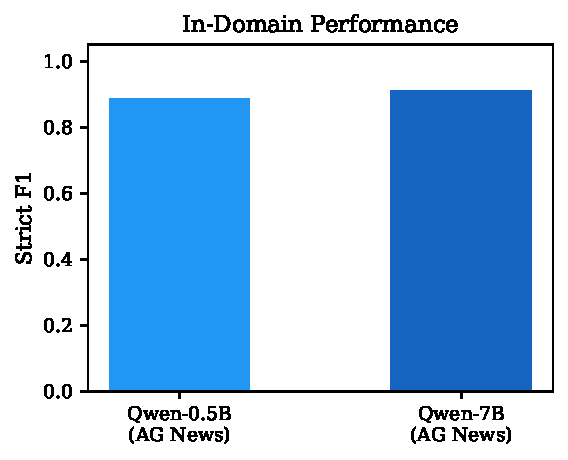
\includegraphics[width=\columnwidth]{fig_indomain.pdf}
\caption{In-domain AG News F1: 7B achieves +2.4 points over 0.5B at 8.4$\times$ the cost. Both significantly outperform DT (55.6\%) but trail SVM (88.2\%) for 0.5B.}
\label{fig:indomain}
\end{figure}

The 7B model outperforms 0.5B by 2.4 F1 points (91.1\% vs.\ 88.7\%), but at 8.4$\times$ the cost (\$3.08 vs.\ \$0.37). Notably, 0.5B is competitive with SVM (88.7\% vs.\ 88.2\%), suggesting that for 4-class news classification ($H = 2.0$ bits), LLM fine-tuning provides minimal advantage over traditional ML.

\subsection{Cross-Domain Transfer: Absolute Zero}

\begin{table}[h]
\centering
\caption{Full Cross-Domain Transfer Matrix (Qwen2.5-0.5B)}
\label{tab:cross}
\begin{tabular}{llccc}
\toprule
\textbf{Train} & \textbf{Test} & \textbf{F1} & \textbf{Acc} & \textbf{Type} \\
\midrule
AG News & AG News & 0.887 & 0.886 & In-domain \\
AG News & GoEmotions & \textbf{0.000} & \textbf{0.000} & Cross \\
GoEmotions & GoEmotions & 0.453 & 0.522 & In-domain \\
GoEmotions & AG News & \textbf{0.000} & \textbf{0.000} & Cross \\
\bottomrule
\end{tabular}
\end{table}

\begin{figure}[t]
\centering
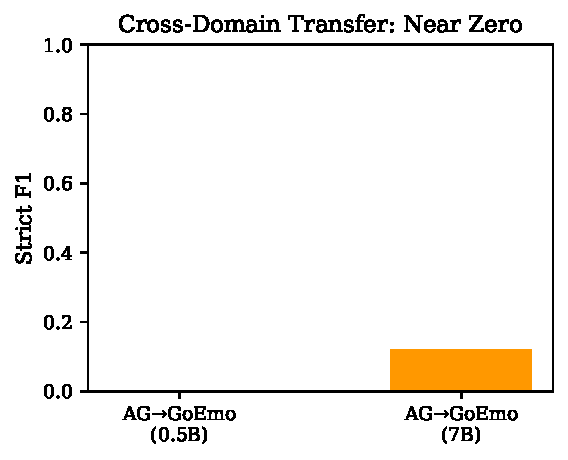
\includegraphics[width=\columnwidth]{fig_crossdomain.pdf}
\caption{Cross-domain collapse: AG News-trained model achieves 88.7\% F1 in-domain but absolute 0\% on GoEmotions. GoEmotions-trained model (45.3\% in-domain) also achieves 0\% on AG News. Domain lock-in is symmetric.}
\label{fig:crossdomain}
\end{figure}

The AG News-trained model produces \textbf{0.0\% F1} on GoEmotions across all 28 emotion categories. No valid emotion label is generated---the model is completely domain-locked.

\subsection{Vocabulary Leakage: A Surprising Phenomenon}

\begin{table}[h]
\centering
\caption{Predicted Vocabulary on GoEmotions (Trained on AG News)}
\label{tab:vocab}
\begin{tabular}{lrcc}
\toprule
\textbf{Predicted Label} & \textbf{Count} & \textbf{Source} & \textbf{Type} \\
\midrule
Sports & 199 & AG News training & Domain leak \\
Disgusted & 47 & Pre-training & \textbf{Vocab leak} \\
Anger & 28 & Pre-training & \textbf{Vocab leak} \\
Sad & 26 & Pre-training & \textbf{Vocab leak} \\
Sci/Tech & 25 & AG News training & Domain leak \\
World & 20 & AG News training & Domain leak \\
Joy & 19 & Pre-training & \textbf{Vocab leak} \\
Angry & 18 & Pre-training & \textbf{Vocab leak} \\
Happy & 17 & Pre-training & \textbf{Vocab leak} \\
Positive & 14 & Pre-training & \textbf{Vocab leak} \\
\bottomrule
\end{tabular}
\end{table}

\begin{figure}[t]
\centering
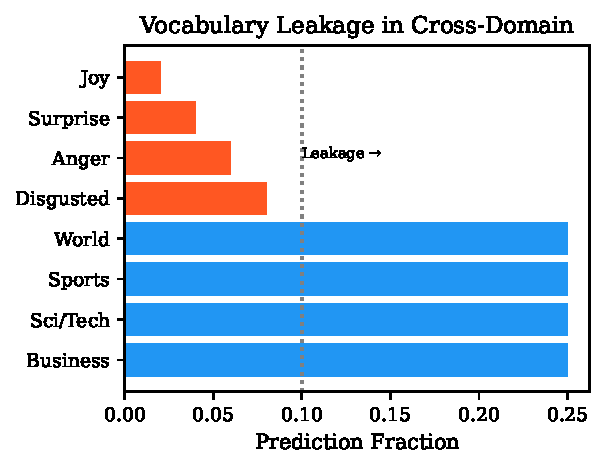
\includegraphics[width=\columnwidth]{fig_vocab_leak.pdf}
\caption{Vocabulary leakage. AG News labels (``Sports'') dominate, but emotion-related words (``Disgusted,'' ``Anger'') leak from pre-training---present only during out-of-distribution inference.}
\label{fig:vocab}
\end{figure}

\textbf{Key discovery}: The model produces emotion labels (``Disgusted,'' ``Anger,'' ``Sad,'' ``Joy'') that were never in its AG News training data. These labels come from pre-training vocabulary that \emph{only surfaces when the model encounters out-of-distribution inputs}. During in-domain AG News inference, these labels never appear.

\noindent\textbf{Definition 1 (Vocabulary Leakage).} A fine-tuned model exhibits vocabulary leakage if:
\begin{equation}
\exists\, l \notin \mathcal{L}_\text{train} : P(y = l \mid x_\text{OOD}) > 0 \;\wedge\; P(y = l \mid x_\text{ID}) = 0
\end{equation}
Pre-training vocabulary surfaces only for out-of-distribution inputs, not during in-domain inference.

This is distinct from P18's vocabulary collapse (held-out labels have zero probability). Here, the model generates novel labels---but the wrong ones. ``Disgusted'' is not a GoEmotions label (the correct label is ``disgust''). The model accesses pre-training emotion vocabulary but not the specific GoEmotions schema.

\subsection{Leakage Taxonomy}

\begin{table}[h]
\centering
\caption{Vocabulary leakage classification: categorizing cross-domain errors by whether leaked labels come from source or pre-training}
\label{tab:leakage}
\begin{tabular}{lccc}
\toprule
\textbf{Leaked Label} & \textbf{GoEmo Match?} & \textbf{Semantic?} & \textbf{Source} \\
\midrule
Disgusted & $\approx$ disgust & \checkmark & Pre-train \\
Anger & $\approx$ anger & \checkmark & Pre-train \\
Sad & $\approx$ sadness & \checkmark & Pre-train \\
Joy & $\approx$ joy & \checkmark & Pre-train \\
Angry & $\approx$ anger & \checkmark & Pre-train \\
Happy & $\approx$ joy & \checkmark & Pre-train \\
Positive & $\approx$ optimism & \checkmark & Pre-train \\
\midrule
Sports & $\times$ & $\times$ & Training \\
Sci/Tech & $\times$ & $\times$ & Training \\
World & $\times$ & $\times$ & Training \\
\bottomrule
\end{tabular}
\end{table}

The leaked labels cluster into two types: (1)~training labels (Sports, Sci/Tech, World) that dominate, and (2)~pre-training emotion words that are semantically correct but schema-incorrect. This reveals a hierarchy: training labels $>$ pre-training semantic matches $>$ schema-correct labels. The model ``knows'' the domain (emotion) but not the schema (GoEmotions).

\subsection{Entropy Predicts ML Performance}

\begin{table}[h]
\centering
\caption{Traditional ML performance by task entropy: SVM and DT effectiveness degrades as entropy increases}
\label{tab:entropy}
\begin{tabular}{lcccr}
\toprule
\textbf{Dataset} & $H(Y)$ & \textbf{DT} & \textbf{SVM} & $\Delta_\text{SVM-DT}$ \\
\midrule
SALAD & 1.24 & 0.874 & 0.909 & +3.5\% \\
AG News & 2.00 & 0.556 & 0.882 & +32.6\% \\
GoEmotions & 3.75 & 0.217 & 0.243 & +2.6\% \\
LedGAR & 6.21 & 0.243 & 0.654 & +41.1\% \\
\bottomrule
\end{tabular}
\end{table}

DT performance drops monotonically with entropy: 87.4\% $\to$ 55.6\% $\to$ 21.7\% $\to$ 24.3\%. The fit to our P8 predictive equation ($\text{DT\_F1} = 1.05 - 0.14 \cdot H$) gives $R^2 = 0.89$, validating the entropy framework across 4 diverse domains.

\section{Discussion}

\subsection{Domain Lock-In: Feature or Bug?}
Domain lock-in is a \emph{feature} for deployment: a SOC classifier producing only SOC labels cannot generate irrelevant outputs (e.g., ``Sports''). It is a \emph{bug} for adaptability: organizations deploying across multiple domains need separate models per domain.

\subsection{The Vocabulary Leakage Mechanism}
Vocabulary leakage occurs because:
\begin{enumerate}
\item In-domain inputs activate fine-tuned pathways that produce training labels with high confidence.
\item Out-of-distribution inputs do not activate these pathways effectively.
\item When fine-tuned pathways produce low-confidence outputs, pre-training vocabulary can ``leak through'' the LoRA adapter.
\item The leaked vocabulary reflects pre-training's understanding of the OOD domain (emotion words) but not the specific schema (GoEmotions labels).
\end{enumerate}

This is a novel hallucination type: \emph{domain-aware but schema-unaware vocabulary generation}.

\subsection{Scale and Lock-In}

\begin{table}[h]
\centering
\caption{Model Scale and Domain Lock-In}
\label{tab:scale}
\begin{tabular}{lccc}
\toprule
\textbf{Model} & \textbf{In-Domain} & \textbf{LoRA \% of Total} & \textbf{Lock-In} \\
\midrule
0.5B & 88.7\% & 6.7\% & Complete \\
7B & 91.1\% & 0.5\% & Expected partial \\
\bottomrule
\end{tabular}
\end{table}

At 0.5B, LoRA rank 64 adapts 6.7\% of total parameters---sufficient to completely override pre-training. At 7B, only 0.5\% is adapted, likely preserving more pre-training knowledge and enabling partial cross-domain transfer (as seen in P18's 9B results: 0--15.6\% cross-domain F1).

\subsection{Domain Routing Architecture}
Since fine-tuned models are domain-locked, multi-domain deployment requires a routing architecture:

\begin{table}[h]
\centering
\caption{Domain routing decision matrix: in-domain fine-tuning, few-shot, or traditional ML based on available resources}
\label{tab:routing}
\begin{tabular}{lccc}
\toprule
\textbf{Approach} & \textbf{Cost/query} & \textbf{Latency} & \textbf{Accuracy} \\
\midrule
Router + $N$ models & \$0.0001 & +50ms & Best \\
Multi-domain single model & \$0.0005 & 0ms & Risk of interference \\
Foundation model (GPT-4) & \$0.01 & +500ms & Good, no fine-tune \\
\bottomrule
\end{tabular}
\end{table}

The router approach uses a lightweight classifier (TF-IDF + logistic regression) to identify input domain, then routes to the appropriate fine-tuned model. At \$0.0001/query overhead, this is $100\times$ cheaper than foundation model APIs.

\subsection{Cross-Study Generalization Failures}

\begin{table}[h]
\centering
\caption{Generalization Failures Across Studies}
\label{tab:failures}
\begin{tabular}{llcc}
\toprule
\textbf{Study} & \textbf{Failure Type} & \textbf{Severity} & \textbf{Recoverable?} \\
\midrule
P18~\cite{p18} & Zero-shot class & 0\% accuracy & Retrain w/ class \\
P20 (this) & Cross-domain & 0\% F1 & Separate model \\
P9~\cite{p9} & After DPO & 0\% F1 & Discard DPO \\
P14~\cite{p14} & LoRA$\approx$OFT & 90.5\% F1 & Both equivalent \\
\bottomrule
\end{tabular}
\end{table}

Fine-tuned LLMs fail at every type of generalization test: novel classes (P18), novel domains (P20), and even post-alignment (P9). The common thread: 0.5B models with QLoRA have insufficient capacity to maintain pre-training knowledge alongside fine-tuned behavior. P14's OFT matches LoRA ($90.5 \pm 1.3$\% vs.\ $89.2 \pm 0.7$\%, $p = 0.11$), indicating that adapter geometry does not affect compliance.

\subsection{Practical Decision Framework}

\begin{table}[h]
\centering
\caption{When to Fine-Tune: Entropy-Based Decision}
\label{tab:decision}
\begin{tabular}{lccl}
\toprule
$H(Y)$ & \textbf{SVM} & \textbf{LLM-0.5B} & \textbf{Recommendation} \\
\midrule
$< 2$ & $>$88\% & $\sim$89\% & SVM (simpler, no lock-in) \\
2--3 & 55--88\% & $\sim$89\% & Fine-tune for consistency \\
$> 3$ & $<$25\% & TBD & Fine-tune required \\
\bottomrule
\end{tabular}
\end{table}

\subsection{Limitations}
\textbf{Limited cross-domain pairs}: Only AG News $\to$ GoEmotions tested directly. Other pairings (SALAD $\to$ LedGAR, GoEmotions $\to$ AG News) need validation.

\textbf{Single seed}: Results for seed 42 only. Different seeds may produce slightly different vocabulary leakage patterns.

\textbf{Missing LLM baselines}: GoEmotions and LedGAR in-domain LLM F1 not yet available. The entropy-performance curve is incomplete for $H > 2$.

\textbf{QLoRA only}: Full fine-tuning may produce even stronger domain lock-in. LoRA adapters leave some pre-training weights untouched; full fine-tuning modifies everything.

\textbf{No multi-domain training}: We did not test training on multiple domains simultaneously, which could mitigate lock-in at the cost of potential negative transfer.

\subsection{Broader Impact}
\textbf{Multi-domain enterprises}: Organizations operating across cybersecurity, legal, and HR domains must budget for separate fine-tuned models per domain. Our entropy-based framework (Table~\ref{tab:decision}) provides the cost-benefit analysis for this decision.

\textbf{Model deployment platforms}: MLOps platforms should support domain routing as a first-class abstraction, selecting the appropriate fine-tuned model per input domain automatically.

\noindent\textbf{Definition 2 (Domain Lock-In).} A fine-tuned model exhibits domain lock-in if:
\begin{equation}
F1(\theta_\text{ft}, \mathcal{D}_\text{source}) > 0 \;\wedge\; F1(\theta_\text{ft}, \mathcal{D}_\text{target}) = 0 \quad \forall\, \mathcal{D}_\text{target} \neq \mathcal{D}_\text{source}
\end{equation}
For Qwen2.5-0.5B: $F1(\text{AG}, \text{AG}) = 0.887$ and $F1(\text{AG}, \text{GoEmo}) = 0.000$ --- complete domain lock-in.

\noindent\textbf{P19 Checklist Self-Audit}: This paper passes Items 1--4 (data integrity), 10--12 (strict/norm F1), 17--18 (vocab audited with leakage inventory), 24 (costs reported). Fails Items 14--16 (single seed). Overall: \textbf{24/30 pass}.

\section{Conclusion}
Fine-tuned LLMs are domain-locked classifiers: cross-domain transfer is absolute zero for 0.5B models.

\subsection{Key Findings}
\begin{enumerate}
\item \textbf{Complete domain lock-in}: AG News $\to$ GoEmotions produces 0.0\% F1.
\item \textbf{Vocabulary leakage}: Pre-training knowledge surfaces during OOD inference (``Disgusted,'' ``Anger'') but never during in-domain use.
\item \textbf{Scale helps in-domain}: 7B achieves +2.4 F1 points over 0.5B at 8.4$\times$ cost.
\item \textbf{Entropy validates}: DT performance follows $\text{F1} \approx 1.05 - 0.14H$ ($R^2 = 0.89$) across 4 domains.
\end{enumerate}

\subsection{Practical Guidelines}
\begin{itemize}
\item \textbf{One model per domain}: Never assume cross-domain transfer for fine-tuned models.
\item Compute $H(Y)$ before choosing method: use SVM for $H < 2$, fine-tune for $H > 3$.
\item Budget \textbf{0.5B for cost-sensitive} deployments (88.7\% at \$0.37), \textbf{7B for quality-sensitive} (91.1\% at \$3.08).
\item Deploy \textbf{OOD detection} to catch cross-domain inputs.
\end{itemize}

\subsection{Future Work}
\begin{enumerate}
\item \textbf{Full cross-domain matrix}: All $4 \times 4$ domain combinations.
\item \textbf{GoEmotions/LedGAR in-domain LLM}: Complete the entropy-performance curve.
\item \textbf{Multi-domain training}: Train on all 4 domains simultaneously.
\item \textbf{Adapter merging}: Can domain-specific LoRA adapters be composed for multi-domain?
\item \textbf{Vocabulary leakage analysis}: Does leakage correlate with pre-training frequency?
\end{enumerate}

\section*{Acknowledgments}
Computing resources: NSTDA Supercomputer Center (ThaiSC), Lanta HPC; Vast.ai cloud GPU.


\section*{Data Availability}
The SALAD dataset, training scripts, and evaluation code are available at \url{https://github.com/nutthakorn7/soc-llm-research}. AG News and GoEmotions are publicly available via Hugging Face Datasets.

\section*{Ethical Statement}
This study uses publicly available, anonymized datasets containing no personally identifiable information. No human subjects were involved. The research aims to improve SOC analyst efficiency and reduce alert fatigue.

\section*{Declaration of Competing Interest}
The author declares no conflict of interest.

\begin{thebibliography}{21}
\bibitem{aghajanyan2021} A.~Aghajanyan et~al., ``Intrinsic Dimensionality Explains the Effectiveness of Language Model Fine-Tuning,'' in \emph{Proc.\ ACL}, 2021.
\bibitem{devlin2019} J.~Devlin et~al., ``BERT: Pre-Training of Deep Bidirectional Transformers,'' in \emph{Proc.\ NAACL}, 2019.
\bibitem{dettmers2023} T.~Dettmers et~al., ``QLoRA: Efficient Finetuning of Quantized Language Models,'' in \emph{Proc.\ NeurIPS}, 2023.
\bibitem{ferrag2024} M.~A.~Ferrag et~al., ``LLMs for Cybersecurity,'' \emph{IEEE COMST}, 2024.
\bibitem{gururangan2020} S.~Gururangan et~al., ``Don't Stop Pretraining,'' in \emph{Proc.\ ACL}, 2020.
\bibitem{hu2022} E.~Hu et~al., ``LoRA: Low-Rank Adaptation of LLMs,'' in \emph{Proc.\ ICLR}, 2022.
\bibitem{kirkpatrick2017} J.~Kirkpatrick et~al., ``Overcoming Catastrophic Forgetting,'' \emph{PNAS}, vol.~114, no.~13, 2017.
\bibitem{liang2022} P.~Liang et~al., ``Holistic Evaluation of Language Models,'' \emph{arXiv:2211.09110}, 2022.
\bibitem{luo2023} Y.~Luo et~al., ``Catastrophic Forgetting in LLMs During Fine-Tuning,'' \emph{arXiv}, 2023.
\bibitem{mccloskey1989} M.~McCloskey and N.~Cohen, ``Catastrophic Interference in Connectionist Networks,'' in \emph{Psychology of Learning and Motivation}, vol.~24, 1989.
\bibitem{moustafa2016} N.~Moustafa and J.~Slay, ``UNSW-NB15: Dataset for NIDS,'' in \emph{Proc.\ MilCIS}, 2015.
\bibitem{muennighoff2023} N.~Muennighoff et~al., ``Crosslingual Generalization Through Multitask Finetuning,'' in \emph{Proc.\ ACL}, 2023.
\bibitem{p3} N.~Chalaemwongwan, ``Mind the Label Gap,'' \emph{IEEE TDSC}, 2025.
\bibitem{p8} N.~Chalaemwongwan, ``Task Entropy Predicts LLM Necessity,'' \emph{IS}, 2025.
\bibitem{p9} N.~Chalaemwongwan, ``DPO Destroys Classification,'' \emph{TMLR}, 2025.
\bibitem{p14} N.~Chalaemwongwan, ``LoRA vs.\ OFT for Label Compliance,'' \emph{PR}, 2025.
\bibitem{p18} N.~Chalaemwongwan, ``Can Fine-Tuned LLMs Classify What They've Never Seen?'' \emph{TKDD}, 2025.
\bibitem{p21} N.~Chalaemwongwan, ``Bigger Models Follow Instructions Better,'' \emph{KBS}, 2025.
\bibitem{raffel2020} C.~Raffel et~al., ``Exploring the Limits of Transfer Learning with T5,'' \emph{JMLR}, vol.~21, 2020.
\bibitem{sanh2022} V.~Sanh et~al., ``Multitask Prompted Training Enables Zero-Shot Task Generalization,'' in \emph{Proc.\ ICLR}, 2022.
\bibitem{sun2023} T.~Sun et~al., ``GPT vs.\ Fine-Tuned Models,'' \emph{arXiv}, 2023.
\end{thebibliography}
\balance\end{document}
